\section{Gradient-based opacity weighting}\label{Sec:Gow}
Another task was to implement gradient-based opacity weighting in our raycaster.
We used the gradient-based opacity as described in Levoy’s paper.
Gradient-based opacity is useful when there is more than one type of  material in the scene. 
Gradient-based opacity can then be used to display or hide certain materials.
With this function we can compute the new opacity value for each pixel:
\[ \tau(i) = |\bigtriangledown f_{i}| \left\{
  \begin{array}{lr}
   \tau_{min} (\frac{ f_{max}- f_{i}}{ f_{max}- f_{min}}) +\tau_{max}( \frac{ f_{i}- f_{min}}{ f_{max}- f_{min}})  & : f_{min} \leq f_{i}  \leq f_{max} \\
    0 & : otherwise 
  \end{array}
\right.
\] 
Because we do not know these values, we have made a settings box that enables users to easily play with those values.
In figure~\ref{fig:gradient_settings} you can see those settings. 
As you can see we added another option: Factor. 
By changing the factor, the user can increase or decrease the effect of the gradient-based opacity weighting function.
\begin{figure}[H]
	\centering
		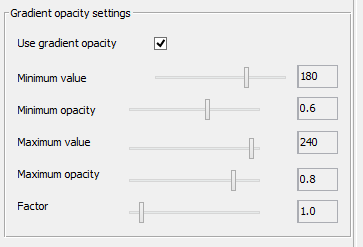
\includegraphics[width=0.4\textwidth]{gradient_settings}
		\caption{Settings for the gradient-based opacity weighting}
	\label{fig:gradient_settings}
\end{figure}